\documentclass[xcolor=table]{beamer}
% generated by Madoko, version 1.1.3
%mdk-data-line={1}


\usepackage[heading-base={2},section-num={False},bib-label={hide},fontspec={True}]{madoko2}
%mdk-data-line={1;out\presentation.mdk:79}

    \ifbeamer\relax\else
      \providecommand{\usetheme}[2][]{}
      \providecommand{\usecolortheme}[2][]{}
      \providecommand{\usefonttheme}[2][]{}
      \providecommand{\pause}[1][]{}
      \providecommand{\AtBeginSection}[2][]{}
      \providecommand{\AtBeginSubsection}[2][]{}
      \providecommand{\AtBeginSubsubsection}[2][]{}
      \providecommand{\AtBeginPart}[2][]{}
      \providecommand{\AtBeginLecture}[2][]{}
      \providecommand{\theoremstyle}[2][]{}
      \makeatletter
      \def\newtheorem{\@ifstar\newtheoremx\newtheoremx}
      \makeatother
      \providecommand{\newtheoremx}[3][]{}{}
    \fi
%mdk-data-line={1;out\presentation.mdk:96}

    \ifbeamer\usetheme[]{singapore}\fi
\begin{document}



%mdk-data-line={9}
%mdk-data-line={9}
%mdk-data-line={10}
\mdxtitleblockstart{}
%mdk-data-line={10}
\mdxtitle{{\mdfontsize{3em}\mdline{10}Particiones balanceadas de conjuntos geometricos 3 coloreados en el plano}}%mdk
\mdxauthorstart{\Large{}
%mdk-data-line={15}
\mdxauthorname{{\mdfontsize{1.4em}\mdline{15}+@Bereg201521}}%mdk

%mdk-data-line={18}
\mdxauthoraddress{\mdline{18}Microsoft Research}%mdk

%mdk-data-line={21}
\mdxauthoremail{\mdline{21}daan@microsoft.com}%mdk
}\mdxauthorend\mdtitleauthorrunning{}{}\mdxtitleblockend%mdk

%mdk-data-line={12}
\begin{mdframe}%mdk

\frametitle{Contenido}\label{heading-sec-contenido}%mdk%mdk
\mdline{13}
\begin{mdtoc}%mdk

\begin{mdtocblock}%mdk

\mdtocitemx{sec-contenido}{\mdref{sec-contenido}{1.\hspace*{0.5em}Contenido}}%mdk

\mdtocitemx{sec-definiciones}{\mdref{sec-definiciones}{2.\hspace*{0.5em}Definiciones}}%mdk

\mdtocitemx{sec-equiparticion}{\mdref{sec-equiparticion}{3.\hspace*{0.5em}Equiparticion}}%mdk

\mdtocitemx{sec-celdas-el-arreglos-coloreados}{\mdref{sec-celdas-el-arreglos-coloreados}{4.\hspace*{0.5em}Celdas el arreglos coloreados}}%mdk

\begin{mdtocblock}%mdk

\mdtocitemx{sec-en-el-plano}{\mdref{sec-en-el-plano}{4.1.\hspace*{0.5em}En el plano}}%mdk

\mdtocitemx{sec-en-dimensiones-ms-grandes}{\mdref{sec-en-dimensiones-ms-grandes}{4.2.\hspace*{0.5em}En dimensiones más grandes}}%mdk
%mdk
\end{mdtocblock}%mdk

\mdtocitemx{sec-conjunto-de-puntos-3-coloreados-y-cuas-balanceadas}{\mdref{sec-conjunto-de-puntos-3-coloreados-y-cuas-balanceadas}{5.\hspace*{0.5em}Conjunto de puntos 3 coloreados y cuñas balanceadas}}%mdk

\mdtocitemx{sec-particiones-balanceadas-en-curvas-cerradas-de-jordan}{\mdref{sec-particiones-balanceadas-en-curvas-cerradas-de-jordan}{6.\hspace*{0.5em}Particiones balanceadas en curvas cerradas de Jordan}}%mdk

\mdtocitemx{sec-l-lineas-en-el--lattice-}{\mdref{sec-l-lineas-en-el--lattice-}{7.\hspace*{0.5em}$L$-lineas en el \emph{lattice}}}%mdk
%mdk
\end{mdtocblock}%mdk
%mdk
\end{mdtoc}%mdk
%mdk
\end{mdframe}\label{sec-contenido}%mdk%mdk

%mdk-data-line={15}
\begin{mdframe}%mdk

\frametitle{Definiciones}\label{heading-sec-definiciones}%mdk%mdk

%mdk-data-line={16}
\begin{mdbmarginx}{1ex}{0pt}{1ex}{0pt}%mdk
%mdk-data-line={17}
\begin{onlyenv}<+->%mdk
\noindent\mdline{17}\textbf{Definition~1.} \mdbr
\mdline{17}  Sea \mdline{17}$S$\mdline{17} un conjunto finitos de objetos geometricos particionados en clases o \mdline{17}\emph{colores}\mdline{17}.
  Sea \mdline{18}$S'\subseteq S$\mdline{18} decimos que esta \mdline{18}\textbf{balanceado}\mdline{18} si contiene la misma cantidad de elementos
  de \mdline{19}$S$\mdline{19} de cada uno de los colores.%mdk
\end{onlyenv}%mdk%mdk
\end{mdbmarginx}%mdk

%mdk-data-line={22}
\begin{mdbmarginx}{1ex}{0pt}{1ex}{0pt}%mdk
%mdk-data-line={23}
\begin{onlyenv}<+->%mdk
\noindent\mdline{23}\textbf{Definition~2.} ({\itshape Arreglo Simple})\mdbr
\mdline{23}  Dado el arreglo, este no contiene lineas paralelas y no mas de dos lineas intersectan
  en un punto%mdk
\end{onlyenv}%mdk%mdk
\end{mdbmarginx}%mdk
%mdk
\end{mdframe}\label{sec-definiciones}%mdk%mdk

%mdk-data-line={29}
\begin{mdframe}%mdk

\frametitle{Equiparticion}\label{heading-sec-equiparticion}%mdk%mdk
\begin{mdtabular}{2}{\dimeval{(\linewidth-\dimwidth{0.50})/1}}{0pt}%mdk
\begin{tabular}{ll}

%mdk-data-line={32}
\begin{mdcolumn}%mdk
\begin{mdblock}{vertical-align=middle,width=\dimwidth{0.50}}%mdk
%mdk-data-line={33}
\noindent\mdline{33}Dado un conjunto con \mdline{33}$2n$\mdline{33} puntos rojos y \mdline{33}$2m$\mdline{33} azules en posición general en el plano.
Siempre exite una linea \mdline{34}$l$\mdline{34} que divide al plano con \mdline{34}$n$\mdline{34} puntos rojos y \mdline{34}$m$\mdline{34} azules
cada mitad.%mdk%mdk
\end{mdblock}%mdk
\end{mdcolumn}%mdk
&
%mdk-data-line={37}
\begin{mdcolumn}%mdk
\begin{mdblock}{width=\dimavailable}%mdk
%mdk-data-line={38}
\noindent\mdline{38}\mdinline{vertical-align=middle}{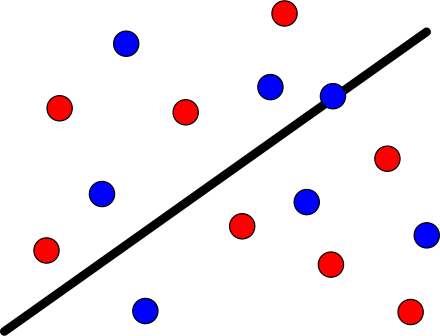
\includegraphics[keepaspectratio=true,width=\dimmin{}{\dimwidth{0.90}}]{images/Discrete_ham_sandwich_cut}{}}\mdline{38}%mdk%mdk
\end{mdblock}%mdk
\end{mdcolumn}%mdk
\\
\end{tabular}\end{mdtabular}
%mdk
\end{mdframe}\label{sec-equiparticion}%mdk%mdk

%mdk-data-line={46}
\begin{mdframe}%mdk

%mdk-data-line={47}
\noindent\mdline{47}  Es posible que dado un conjunto tricolor de puntos en plano no se pueda encontrar
  ninguna linea \mdline{48}\emph{no trivial}\mdline{48} que divida al plano%mdk
%mdk
\end{mdframe}%mdk

%mdk-data-line={50}
\begin{mdframe}%mdk

%mdk-data-line={51}
\noindent\mdline{51}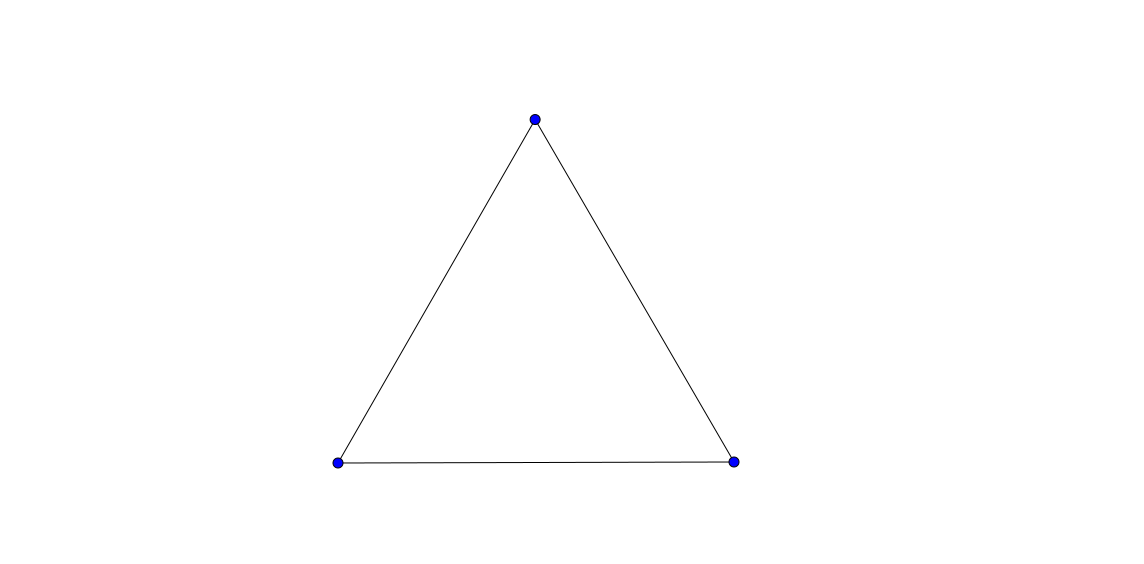
\includegraphics[keepaspectratio=true,width=\dimwidth{1.00},height=\dimheight{1.00}]{images/non_trivial_cut00}{}%mdk
%mdk
\end{mdframe}%mdk

%mdk-data-line={53}
\begin{mdframe}%mdk

%mdk-data-line={54}
\noindent\mdline{54}\includegraphics[keepaspectratio=true,width=\dimwidth{1.00},height=\dimheight{1.00}]{images/non_trivial_cut01}{}%mdk
%mdk
\end{mdframe}%mdk

%mdk-data-line={56}
\begin{mdframe}%mdk

%mdk-data-line={57}
\noindent\mdline{57}\includegraphics[keepaspectratio=true,width=\dimwidth{1.00},height=\dimheight{1.00}]{images/non_trivial_cut02}{}%mdk
%mdk
\end{mdframe}%mdk

%mdk-data-line={59}
\begin{mdframe}%mdk

%mdk-data-line={60}
\noindent\mdline{60}\includegraphics[keepaspectratio=true,width=\dimwidth{1.00},height=\dimheight{1.00}]{images/non_trivial_cut03}{}%mdk
%mdk
\end{mdframe}%mdk

%mdk-data-line={62}
\begin{mdframe}%mdk

%mdk-data-line={63}
\noindent\mdline{63}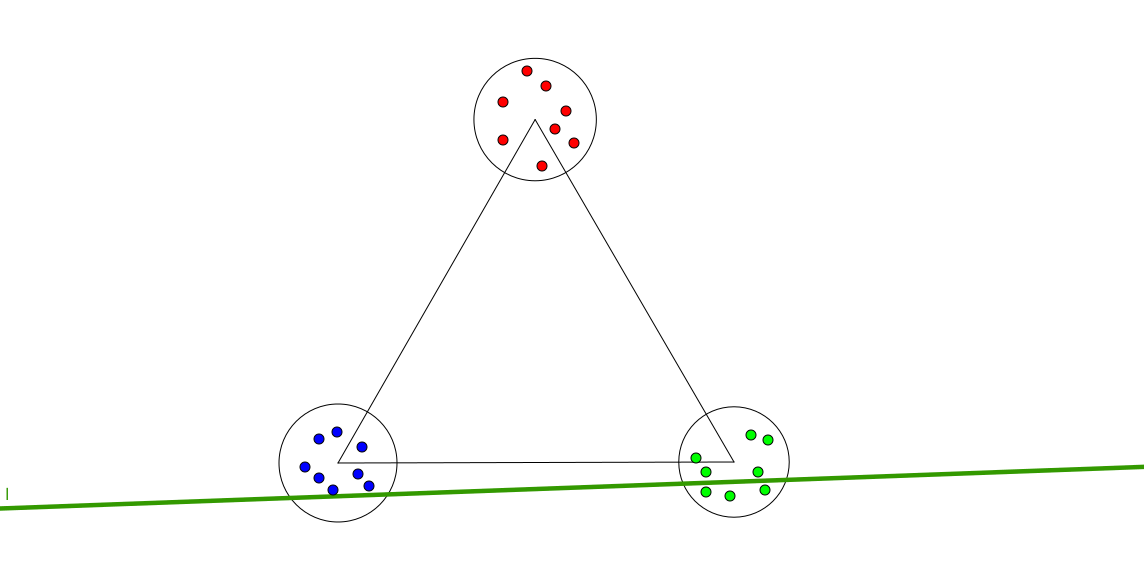
\includegraphics[keepaspectratio=true,width=\dimwidth{1.00},height=\dimheight{1.00}]{images/non_trivial_cut04}{}%mdk
%mdk
\end{mdframe}%mdk

%mdk-data-line={67}
\begin{mdframe}%mdk

\frametitle{Celdas el arreglos coloreados}\label{heading-sec-celdas-el-arreglos-coloreados}%mdk%mdk
%mdk
\end{mdframe}\label{sec-celdas-el-arreglos-coloreados}%mdk%mdk

%mdk-data-line={69}
\begin{mdframe}%mdk

\frametitle{En el plano}\label{heading-sec-en-el-plano}%mdk%mdk

%mdk-data-line={70}
\begin{mdbmarginx}{1ex}{0pt}{1ex}{0pt}%mdk
%mdk-data-line={71}
\noindent\mdline{71}\textbf{Theorem~1.} \mdbr
\mdline{71}  Sea \mdline{71}$L$\mdline{71} un conjunto 3 coloreado en el plano que induce un arreglo simple \mdline{71}$A(L)$\mdline{71}, talque
que cada color aparece al menos una ves. Entonces existe una \mdline{72}\emph{cara completa}\mdline{72} en \mdline{72}$A(L)$%mdk%mdk
\end{mdbmarginx}%mdk

%mdk-data-line={75}
\begin{mdbmarginx}{1ex}{0pt}{1ex}{0pt}%mdk
%mdk-data-line={76}
\noindent\mdline{76}\textbf{Lemma~1.} \mdbr
\mdline{76} Considera un ciclo simple donde cada vertice es coloreado con rojo, verde o azul. Entonces
 \mdline{77}$n_{rg} \equiv n_{rb} \equiv n_{gb} \mod 2$%mdk%mdk
\end{mdbmarginx}%mdk
%mdk
\end{mdframe}\label{sec-en-el-plano}%mdk%mdk

%mdk-data-line={80}
\begin{mdframe}%mdk

\frametitle{En dimensiones más grandes}\label{heading-sec-en-dimensiones-ms-grandes}%mdk%mdk

%mdk-data-line={81}
\begin{mdbmarginx}{1ex}{0pt}{1ex}{0pt}%mdk
%mdk-data-line={82}
\noindent\mdline{82}\textbf{Theorem~2.} \mdbr
\mdline{82}Sea \mdline{82}$L$\mdline{82} un conjunto de \mdline{82}$(d+1)$\mdline{82}-coloreados hyperplanos en \mdline{82}$I\!R^{d}$\mdline{82} que induce un arreglo simple
en \mdline{83}$A(L)$\mdline{83}, donde cada color aparece al menos una vez. Entonces existe una \mdline{83}\emph{cara completa}\mdline{83} en \mdline{83}$A(L)$%mdk%mdk
\end{mdbmarginx}%mdk

%mdk-data-line={86}
\begin{mdbmarginx}{1ex}{0pt}{1ex}{0pt}%mdk
%mdk-data-line={87}
\noindent\mdline{87}\textbf{Lemma~2.} \mdbr
\mdline{87}Considera una triangulación \mdline{87}$T$\mdline{87} en \mdline{87}$\mathbb{S}^{d-1}$\mdline{87} donde cada vertice es coloreado con un color
\mdline{88}{}[\mdline{88}$d$\mdline{88}]\mdline{88}. Entonces \mdline{88}$n_{s} \equiv 0(mod\ 2)$\mdline{88} para todos los \mdline{88}\emph{buenos tipos}\mdline{88} \mdline{88}$S$\mdline{88}, o
\mdline{89}$n_{s} \equiv 1 (mod\ 2)$\mdline{89} para todos los \mdline{89}\emph{buenos tipos}\mdline{89} \mdline{89}$S$\mdline{89}%mdk%mdk
\end{mdbmarginx}%mdk
%mdk
\end{mdframe}\label{sec-en-dimensiones-ms-grandes}%mdk%mdk

%mdk-data-line={92}
\begin{mdframe}%mdk

\frametitle{Conjunto de puntos 3 coloreados y cuñas balanceadas}\label{heading-sec-conjunto-de-puntos-3-coloreados-y-cuas-balanceadas}%mdk%mdk
%mdk
\end{mdframe}\label{sec-conjunto-de-puntos-3-coloreados-y-cuas-balanceadas}%mdk%mdk

%mdk-data-line={94}
\begin{mdframe}%mdk

%mdk-data-line={95}
\begin{mdbmarginx}{1ex}{0pt}{1ex}{0pt}%mdk
%mdk-data-line={96}
\noindent\mdline{96}\textbf{Theorem~3.} \mdbr
\mdline{96}Sea \mdline{96}$S$\mdline{96} un conjunto de puntos 3 coloreado en \mdline{96}$\mathbb{R}^{2}$\mdline{96} en posición general, donde cada
color aparece al menos una vez. Entonces existe un \mdline{97}\textbf{cuña}\mdline{97} que contiene exactamente un punto
de cada color de \mdline{98}$S$%mdk%mdk
\end{mdbmarginx}%mdk
%mdk
\end{mdframe}%mdk

%mdk-data-line={102}
\begin{mdframe}%mdk

%mdk-data-line={103}
\begin{mdbmarginx}{1ex}{0pt}{1ex}{0pt}%mdk
%mdk-data-line={104}
\noindent\mdline{104}\textbf{Theorem~4.} \mdbr
\mdline{104}Sea un conjunto 3 coloreado \mdline{104}\emph{balanceado}\mdline{104} de 6\mdline{104}$n$\mdline{104} puntos en \mdline{104}$\mathbb{R}^{2}$\mdline{104} en posición
general. Entonces existe una \mdline{105}\textbf{cuña}\mdline{105} que contiene exactamente n puntos de cada color de \mdline{105}$S$%mdk%mdk
\end{mdbmarginx}%mdk

%mdk-data-line={108}
\begin{mdbmarginx}{1ex}{0pt}{1ex}{0pt}%mdk
%mdk-data-line={109}
\noindent\mdline{109}\textbf{Corollary~1.} \mdbr
\mdline{109}Sea \mdline{109}$L$\mdline{109} un conjunto 3 coloreado balanceado de 6\mdline{109}$n$\mdline{109} lineas en \mdline{109}$\mathbb{R}^2$\mdline{109} que induce un 
arreglo simple. Entonces, siemple existe un segmento que intersecta exactamente \mdline{110}$n$\mdline{110} lineas
de cada color%mdk%mdk
\end{mdbmarginx}%mdk
%mdk
\end{mdframe}%mdk

%mdk-data-line={116}
\begin{mdframe}%mdk

\frametitle{Particiones balanceadas en curvas cerradas de Jordan}\label{heading-sec-particiones-balanceadas-en-curvas-cerradas-de-jordan}%mdk%mdk
%mdk
\end{mdframe}\label{sec-particiones-balanceadas-en-curvas-cerradas-de-jordan}%mdk%mdk

%mdk-data-line={118}
\begin{mdframe}%mdk

%mdk-data-line={119}
\begin{mdbmarginx}{1ex}{0pt}{1ex}{0pt}%mdk
%mdk-data-line={120}
\noindent\mdline{120}\textbf{Lemma~3.} \mdbr
\mdline{120}Para un entero fijo \mdline{120}$n \geq 2$\mdline{120} cualquier \mdline{120}$k \in \{1,2,...,n\}$\mdline{120} puede ser obtenido desde n
aplicando funciones \mdline{121}$f(x) = \lfloor x \rfloor$\mdline{121} y \mdline{121}$g(x)= n - x$\mdline{121} en a lo más \mdline{121}$2 \log n + O(1)$\mdline{121} tiempo%mdk%mdk
\end{mdbmarginx}%mdk
%mdk
\end{mdframe}%mdk

%mdk-data-line={125}
\begin{mdframe}%mdk

%mdk-data-line={126}
\begin{mdbmarginx}{1ex}{0pt}{1ex}{0pt}%mdk
%mdk-data-line={127}
\noindent\mdline{127}\textbf{Theorem~5.} \mdbr
\mdline{127}Sea \mdline{127}$\gamma$\mdline{127} un curva cerrada de Jordan en el plano, y sea \mdline{127}$P$\mdline{127} un conjunto 3 coloreado balanceado de \mdline{127}$3n$\mdline{127} puntos
en \mdline{128}$\gamma$\mdline{128}. Entonces para cada entero positivo \mdline{128}$k \leq n$\mdline{128} existe un \mdline{128}$2$\mdline{128}-arco conjunto \mdline{128}$P_{k} \subseteq \gamma$\mdline{128} 
que contiene exactamente \mdline{129}$k$\mdline{129} puntos de cada color.%mdk%mdk
\end{mdbmarginx}%mdk
%mdk
\end{mdframe}%mdk

%mdk-data-line={133}
\begin{mdframe}%mdk

\frametitle{$L$-lineas en el \emph{lattice}}\label{heading-sec-l-lineas-en-el--lattice-}%mdk%mdk
%mdk
\end{mdframe}\label{sec-l-lineas-en-el--lattice-}%mdk%mdk

%mdk-data-line={135}
\begin{mdframe}%mdk

%mdk-data-line={136}
\begin{mdbmarginx}{1ex}{0pt}{1ex}{0pt}%mdk
%mdk-data-line={137}
\noindent\mdline{137}\textbf{Definition~3.} ({\itshape L-linea})\mdbr%mdk%mdk
\end{mdbmarginx}%mdk

%mdk-data-line={138}
\begin{mdbmarginx}{1ex}{0pt}{1ex}{0pt}%mdk
%mdk-data-line={139}
\noindent\mdline{139}\textbf{Definition~4.} ({\itshape Posicion general en el Lattice})\mdbr%mdk%mdk
\end{mdbmarginx}%mdk
%mdk
\end{mdframe}%mdk

%mdk-data-line={143}
\begin{mdframe}%mdk

%mdk-data-line={144}
\begin{mdbmarginx}{1ex}{0pt}{1ex}{0pt}%mdk
%mdk-data-line={145}
\noindent\mdline{145}\textbf{Theorem~6.} \mdbr
\mdline{145}  Sea \mdline{145}$S$\mdline{145} un conjunto de puntos 3 coloreado balanceado de \mdline{145}$3n$\mdline{145} puntos en posicion general
  en el plano. Si el cierre convexo es \mdline{146}\emph{monocromatico}\mdline{146} entonces existe un linea de balanceo
  no trivial.%mdk%mdk
\end{mdbmarginx}%mdk
%mdk
\end{mdframe}%mdk

%mdk-data-line={151}
\begin{mdframe}%mdk

%mdk-data-line={152}
\begin{mdbmarginx}{1ex}{0pt}{1ex}{0pt}%mdk
%mdk-data-line={153}
\noindent\mdline{153}\textbf{Theorem~7.} \mdbr
\mdline{153}Sea \mdline{153}$S$\mdline{153} un conjunto 3 coloreado balanceado de \mdline{153}$3n$\mdline{153} puntos en posicion general en el \mdline{153}\emph{lattice}\mdline{153}.
Si el cierre ortogonal convezo de \mdline{154}$S$\mdline{154} es \mdline{154}\emph{monocromatico}\mdline{154}, entonces exita una \mdline{154}$L$\mdline{154}-linea de balanceo
no trivial.%mdk%mdk
\end{mdbmarginx}%mdk
%mdk
\end{mdframe}%mdk%mdk%mdk%mdk


\end{document}
